
\documentclass{ion-gps}

  \usepackage{alltt}
  \usepackage{subfigure}
  \usepackage{graphicx}
  \usepackage{listings}

  \usepackage{amsmath}     % cases environment
  \usepackage{indentfirst} % indent all first paragraphs
  \usepackage{times}

  \usepackage{multirow}
  \usepackage{rotating}
  \usepackage{colortbl}
  \usepackage{xcolor}

  \newcommand{\sideco}{gray}
  \newcommand{\sideso}{1.0}
  \newcommand{\sidect}{gray}
  \newcommand{\sidest}{1.0}
  \newcommand{\sidewidth}{.05in}
  \newcommand{\entco}{gray}
  \newcommand{\entso}{1.00}
  \newcommand{\entct}{gray}
  \newcommand{\entst}{0.95}

  \newcommand{\twidth}{1.15in}
  \newcommand{\dwidth}{2.0in}
  \newcommand{\ewidth}{3.0in}
  \newcommand{\bkup}{-2}
  \newcommand{\execsize}{\scriptsize}
  \newcommand{\sidesize}{\small}

  \newcommand{\gpstkapplication}[1]{\texttt{#1}}
  \newcommand{\gpstkdir}[1]{\texttt{#1}}
  \newcommand{\gpstkclass}[1]{\texttt{#1}}
  \newcommand{\rinexobservable}[1]{\texttt{#1}}

%%%%%%%%%%%%%%%%%%%%%%%%%%%%%%%%%%%%%%%%%%%%%%%%%%%%%%%%%%%%%%%%%%%%%%%%%%%%%%%
% Title
%%%%%%%%%%%%%%%%%%%%%%%%%%%%%%%%%%%%%%%%%%%%%%%%%%%%%%%%%%%%%%%%%%%%%%%%%%%%%%%

\title{\huge\bf Open Signals, Open Software:\\
                Two Years of Collaborative Analysis using \\
                the GPS Toolkit }

\author{R. Benjamin Harris, Timothy Craddock, Tracie Conn, Thomas Gaussiran, 
        Eric Hagen, \\
        Anthony Hughes, Jon Little, Richard Mach, Scot Nelsen, 
        Brent Renfro, Brian Tolman\\ 
        \it{Applied Research Laboratories, The University of Texas at Austin}}

\date{}

\conference{First presented at ION GNSS 2006, Sept. 26--29, 2006, Fort Worth, Texas}


%%%%%%%%%%%%%%%%%%%%%%%%%%%%%%%%%%%%%%%%%%%%%%%%%%%%%%%%%%%%%%%%%%%%%%%%%%%%%%%
% Defines
%%%%%%%%%%%%%%%%%%%%%%%%%%%%%%%%%%%%%%%%%%%%%%%%%%%%%%%%%%%%%%%%%%%%%%%%%%%%%%%

\newcommand{\br}{\mbox{\boldmath $r$}}
\newcommand{\bv}{\mbox{\boldmath $v$}}
\newcommand{\be}{\mbox{\boldmath $e$}}
\newcommand{\bzero}{\mbox{\boldmath $0$}}
\newcommand{\bomega}{\mbox{\boldmath $\omega$}}
\newcommand{\bK}{\mbox{\boldmath $K$}}
\newcommand{\bx}{\mbox{\boldmath $x$}}
\newcommand{\ba}{\mbox{\boldmath $a$}}
\newcommand{\bI}{\mbox{\boldmath $I$}}
\newcommand{\bPhi}{\mbox{\boldmath $\Phi$}}
\newcommand{\bH}{\mbox{\boldmath $H$}}
\newcommand{\bR}{\mbox{\boldmath $R$}}
\newcommand{\bQ}{\mbox{\boldmath $Q$}}
\newcommand{\bP}{\mbox{\boldmath $P$}}

\definecolor{console}{rgb}{0.90,0.90,0.90}
\lstset{basicstyle=\ttfamily, backgroundcolor=\color{console}}


%%%%%%%%%%%%%%%%%%%%%%%%%%%%%%%%%%%%%%%%%%%%%%%%%%%%%%%%%%%%%%%%%%%%%%%%%%%%%%%
% Body
%%%%%%%%%%%%%%%%%%%%%%%%%%%%%%%%%%%%%%%%%%%%%%%%%%%%%%%%%%%%%%%%%%%%%%%%%%%%%%%

\begin{document}

\def\figurename{Fig.}
\def\tablename{Table}

\pagestyle{plain} % Page number on back of paper with hand written in pencil
%\pagestyle{fancy}

\maketitle

\thispagestyle{empty} % empty pagestyle for the title page

\section*{Biography}

R. Benjamin Harris is an Engineering Scientist at \mbox{Applied Research
Laboratories} (ARL:UT). He received a B.S. in Aerospace Engineering from UT Austin (1994), and is a Ph.D. candidate in the same department. He received an M.S. in Aeronautics and Astronautics from \mbox{Stanford (2000)}.

Timothy Craddock is an undergraduate majoring in the Electrical
Engineering at UT Austin.

Tracie Conn is an Engineering Scientist Associate at ARL:UT. She
graduated with a B.S. in Aerospace Engineering from UT Austin (2006).

Thomas Gaussiran is the director of the Space and Geophysics Laboratory
(SGL) at ARL:UT. He received his B.S. in Physics from UT Austin (1988)
and M.S. (1991) and PhD. (1994) from Rice University.

Eric Hagen is an undergraduate in the Aerospace Engineering department
at UT Austin.

Anthony Hughes is an Engineering Scientist Associate at ARL:UT. He
graduated with a B.S. in Computer Science from UT Austin (1995).

Jon Little is a Senior Engineering Scientist at ARL:UT. He obtained a
B.S. (1988) and a M.S. (1990) from Auburn.

Richard Mach is a project lead at ARL:UT.  He has been involved with
GPS applications since 1990.  He holds a B.S. (1990) and M.S. (1992) in Aerospace
Engineering from UT Austin.

Scot Nelsen is an Engineering Scientist at ARL:UT. He earned a B.S. in
Electrical Engineering at UT Austin (1998).

Brent Renfro is a division head at ARL:UT. He has a B.A. in Physics
from Wabash College (1979) and a M.A. in Computer Science from UT
Austin (1983).

Brian Tolman is a Research Scientist at ARL:UT. He holds a
Ph.D. in theoretical physics from UT Austin (1982).

\section*{Abstract}
The GPS Toolkit, or GPSTk, is an open source project that provides a
software suite to the GNSS community. The goal of the project is to
free researchers to focus on research, not lower-level
coding. The suite is composed of a library and a suite of
applications that use that library. The library provides common
routines such as those developed in satellite navigation texts. The
applications support greater depth of functionality to support
research and development. The applications are almost entirely
console based (i.e., without a graphical user interface). They can be
grouped functionally into a number of categories: basic
transformations of time and coordinate systems, observation data
collection and conversion, file comparison and validation, data
editing, ionosphere modeling, and autonomous and relative
positioning. New applications have been added to the suite over the
last year. One new application, \gpstkapplication{DDBase}, can be
used to generate baseline solutions with millimeter level accuracy. The
library has been enhanced in the last year and low level input
and output capability for BINEX data has been added.
Future contributions to the library include support for the
Receiver Independent Exchange Format (RINEX) Version 3 format.

\section*{Introduction}

The goal of the GPSTk project is to provide a
open source library and suite of applications to the satellite
navigation community. GPSTk is available both as source and binaries
for several platforms including Linux, Windows, and Solaris.

The GPSTk can be downloaded over the web through the project
website\cite{gpstkwebsite}. The source is provided under the Lesser
GNU Public License (LGPL). The LGPL grants the user permission to use,
modify, and redistribute GPSTk source code. It does not require that
works based on the GPSTk adopt an open source license. Notably,
commercial projects can adopt the GPSTk without being required to open
their code base.

The project source is organized into a core library and a set of
applications that utilize this library. The emphasis of prior papers
has been to announce the project, describe its purpose, and explain how to use
the library to build new applications\cite{ion:gnss04, lj04}. One
paper delineates how to use the applications in tandem to model the
ionosphere\cite{beacon04}. In contrast to prior papers, this
paper will contain a comprehensive introduction to the GPSTk
applications for general use. In addition, recent enhancements to both
the library and applications will be described.  Recent changes to
project operation will also be documented.

\section*{Project Description}

As a project, the GPSTk has changed significantly since it was
presented at the ION-GNSS-2005. New processes have been implemented to
support both development of code and use of the
applications. For development, the code is now hosted in a shared 
online repository at Source Forge\cite{sourceforge}, and automated testing
is provided by a new framework. Users are now supported with an online collaborative
project site. In addition, a user manual for the GPSTk applications
has been initiated and is publicly available.

\subsection*{Test Process}

As an open source project, the source of the GPSTk is subject to
intermittent updates, contributions, and corrections. The GPSTk
library testing process has been redesigned to build confidence in the
functionality of the library.  The open source nature of the project lends
need to verify that newly submitted or corrected code does not
compromise existing code. Furthermore, extensive GPSTk library testing
assists with verification when porting the library to new platforms or
new development environments. Testing within the GPSTk library is
designed with three distinct goals in mind: testing is repeatable with
a low amount of effort, testing is distributed along with the library
to support both internal regression testing and to assure outside
users and contributors of the quality of the library, and testing is
designed accommodate easy additions to the existing test suite.

GPSTk testing implements tools to both assist in building a
comprehensive testing framework and to evaluate the extent to which
the test suite tests the library. CppUnit \cite{CppUnit}, gcov
\cite{gcov}, and Perl \cite{perl} scripts are tools used in the
implementation of GPSTk testing. CppUnit is an open source C++ unit
testing framework that is used within GPSTk. CppUnit provides the
backbone for the GPSTk test suite by allowing for easy test addition
and manipulation, a clear pass/fail output, and many extra
features. Unit test coverage of the GPSTk library is evaluated by the
GNU test coverage tool gcov. Test coverage is assessed by gcov through
execution of the individual test. gcov provides an easy to read
percentage of lines covered while also providing an in depth
line-by-line analysis of the tested code. By examining the results of
gcov, contributors are able to evaluate the thoroughness of the their
unit tests and the extent of the unit tests already implemented within
the GPSTk.

GPSTk testing is an ongoing process with coverage that is always
expanding. Currently, GPSTk testing covers 40\% of the classes within
the library with an average of 95\% line coverage within each of those
classes.  Future plans include expanding coverage over the library
with the hope of eventually reaching 100\% coverage of classes in the
library.

\subsection*{Online Source Management}
Prior to July 2006, access to the GPSTk source was provided via
compressed snapshots. External contributions were taken via email and
merged with a repository internal to ARL:UT. That process proved to be
labor intensive and prone to errors. Now 

\subsection*{Online Project Documentation}

With the initial release of GPSTk, ARL:UT provided a full copy of the
project's source code to the community but the development
process remained inside ARL:UT.  As the project has evolved, ARL:UT
has been moving to an open development process.  This involved
moving the hosting of the code from our internal storage to a
subversion repository hosted on Sourceforge.  However, as with any
project, there are things that need to get described and documented to
help users and contributors effectively utilize or work on the GPSTk.
Previously, this information was hosted on static web pages on
Sourceforge or in internal documentation.  To support the
collaborative environment, ARL:UT is establishing a GPSTk Wiki site so
that anyone can modify and contribute to this supporting material.


The initial version of the wiki is expected to contain the content of
the static web pages and internal development information.  This
includes the GPSTk overview, instructions, examples, coding style
guides, and development processes.  ARL:UT has selected TWiki
\cite{twiki} for this project and expects to have the wiki on-line by
the end of 2006.  TWiki is an easy to use flexible web based
collaboration platform and knowledge management system.  In addition
to having the ability to handle unstructured content, TWiki contains
features of a structured wiki that can be used to manage structured
content like defect tracking, feature requests, knowledge base, and
document management.  ARL:UT is working toward merging all non-code
structured and unstructured GPSTk content into the wiki. This will
provide an adaptive, comprehensive, and unified source of information
to support the community of GPSTk developers and users.

\section*{Review of the GPSTk applications}

While the library provides basic functions such as those that might be
found in a textbook, the GPSTk applications provide more advanced
capabilities necessary to perform research and development.

The GPSTk applications are often developed to meet specific needs. Because
of this, they may not compile or run under all the platforms for which the
GPSTk library compiles due to platform specific dependencies.

The GPSTk applications are summarized, by group, in
Table~\ref{apptable}. They are sorted loosely into groups by their general 
purpose. Each row describes one GPSTk application or a
set of similar applications. The application is named and
described. An example of how the application is executed on a console
is also provided. More detail can be found for each of these
applications by referring to the GPSTk user
guide. This guide describes the theory of processing behind the GPSTk
applications and contains an alphabetized guide to
each GPSTk application. The guide, still in development as of this
writing, can be downloaded from the GPSTk website\cite{gpstkguide}.
Each group is discussed briefly in the following sections.


%\begin{figure}[htbp]
%  \centering
%  % GNUPLOT: LaTeX picture
\setlength{\unitlength}{0.240900pt}
\ifx\plotpoint\undefined\newsavebox{\plotpoint}\fi
\sbox{\plotpoint}{\rule[-0.200pt]{0.400pt}{0.400pt}}%
\begin{picture}(1500,900)(0,0)
\sbox{\plotpoint}{\rule[-0.200pt]{0.400pt}{0.400pt}}%
\put(140.0,82.0){\rule[-0.200pt]{4.818pt}{0.400pt}}
\put(120,82){\makebox(0,0)[r]{-1}}
\put(1419.0,82.0){\rule[-0.200pt]{4.818pt}{0.400pt}}
\put(140.0,160.0){\rule[-0.200pt]{4.818pt}{0.400pt}}
\put(120,160){\makebox(0,0)[r]{-0.8}}
\put(1419.0,160.0){\rule[-0.200pt]{4.818pt}{0.400pt}}
\put(140.0,238.0){\rule[-0.200pt]{4.818pt}{0.400pt}}
\put(120,238){\makebox(0,0)[r]{-0.6}}
\put(1419.0,238.0){\rule[-0.200pt]{4.818pt}{0.400pt}}
\put(140.0,315.0){\rule[-0.200pt]{4.818pt}{0.400pt}}
\put(120,315){\makebox(0,0)[r]{-0.4}}
\put(1419.0,315.0){\rule[-0.200pt]{4.818pt}{0.400pt}}
\put(140.0,393.0){\rule[-0.200pt]{4.818pt}{0.400pt}}
\put(120,393){\makebox(0,0)[r]{-0.2}}
\put(1419.0,393.0){\rule[-0.200pt]{4.818pt}{0.400pt}}
\put(140.0,471.0){\rule[-0.200pt]{4.818pt}{0.400pt}}
\put(120,471){\makebox(0,0)[r]{ 0}}
\put(1419.0,471.0){\rule[-0.200pt]{4.818pt}{0.400pt}}
\put(140.0,549.0){\rule[-0.200pt]{4.818pt}{0.400pt}}
\put(120,549){\makebox(0,0)[r]{ 0.2}}
\put(1419.0,549.0){\rule[-0.200pt]{4.818pt}{0.400pt}}
\put(140.0,627.0){\rule[-0.200pt]{4.818pt}{0.400pt}}
\put(120,627){\makebox(0,0)[r]{ 0.4}}
\put(1419.0,627.0){\rule[-0.200pt]{4.818pt}{0.400pt}}
\put(140.0,704.0){\rule[-0.200pt]{4.818pt}{0.400pt}}
\put(120,704){\makebox(0,0)[r]{ 0.6}}
\put(1419.0,704.0){\rule[-0.200pt]{4.818pt}{0.400pt}}
\put(140.0,782.0){\rule[-0.200pt]{4.818pt}{0.400pt}}
\put(120,782){\makebox(0,0)[r]{ 0.8}}
\put(1419.0,782.0){\rule[-0.200pt]{4.818pt}{0.400pt}}
\put(140.0,860.0){\rule[-0.200pt]{4.818pt}{0.400pt}}
\put(120,860){\makebox(0,0)[r]{ 1}}
\put(1419.0,860.0){\rule[-0.200pt]{4.818pt}{0.400pt}}
\put(140.0,82.0){\rule[-0.200pt]{0.400pt}{4.818pt}}
\put(140,41){\makebox(0,0){ 0}}
\put(140.0,840.0){\rule[-0.200pt]{0.400pt}{4.818pt}}
\put(400.0,82.0){\rule[-0.200pt]{0.400pt}{4.818pt}}
\put(400,41){\makebox(0,0){ 2}}
\put(400.0,840.0){\rule[-0.200pt]{0.400pt}{4.818pt}}
\put(660.0,82.0){\rule[-0.200pt]{0.400pt}{4.818pt}}
\put(660,41){\makebox(0,0){ 4}}
\put(660.0,840.0){\rule[-0.200pt]{0.400pt}{4.818pt}}
\put(919.0,82.0){\rule[-0.200pt]{0.400pt}{4.818pt}}
\put(919,41){\makebox(0,0){ 6}}
\put(919.0,840.0){\rule[-0.200pt]{0.400pt}{4.818pt}}
\put(1179.0,82.0){\rule[-0.200pt]{0.400pt}{4.818pt}}
\put(1179,41){\makebox(0,0){ 8}}
\put(1179.0,840.0){\rule[-0.200pt]{0.400pt}{4.818pt}}
\put(1439.0,82.0){\rule[-0.200pt]{0.400pt}{4.818pt}}
\put(1439,41){\makebox(0,0){ 10}}
\put(1439.0,840.0){\rule[-0.200pt]{0.400pt}{4.818pt}}
\put(140.0,82.0){\rule[-0.200pt]{312.929pt}{0.400pt}}
\put(1439.0,82.0){\rule[-0.200pt]{0.400pt}{187.420pt}}
\put(140.0,860.0){\rule[-0.200pt]{312.929pt}{0.400pt}}
\put(140.0,82.0){\rule[-0.200pt]{0.400pt}{187.420pt}}
\put(1279,820){\makebox(0,0)[r]{Series 1}}
\put(1299.0,820.0){\rule[-0.200pt]{24.090pt}{0.400pt}}
\put(140,471){\usebox{\plotpoint}}
\multiput(140.58,471.00)(0.497,1.493){49}{\rule{0.120pt}{1.285pt}}
\multiput(139.17,471.00)(26.000,74.334){2}{\rule{0.400pt}{0.642pt}}
\multiput(166.58,548.00)(0.497,1.435){49}{\rule{0.120pt}{1.238pt}}
\multiput(165.17,548.00)(26.000,71.430){2}{\rule{0.400pt}{0.619pt}}
\multiput(192.58,622.00)(0.497,1.337){49}{\rule{0.120pt}{1.162pt}}
\multiput(191.17,622.00)(26.000,66.589){2}{\rule{0.400pt}{0.581pt}}
\multiput(218.58,691.00)(0.497,1.142){49}{\rule{0.120pt}{1.008pt}}
\multiput(217.17,691.00)(26.000,56.908){2}{\rule{0.400pt}{0.504pt}}
\multiput(244.58,750.00)(0.497,0.927){49}{\rule{0.120pt}{0.838pt}}
\multiput(243.17,750.00)(26.000,46.260){2}{\rule{0.400pt}{0.419pt}}
\multiput(270.58,798.00)(0.497,0.693){49}{\rule{0.120pt}{0.654pt}}
\multiput(269.17,798.00)(26.000,34.643){2}{\rule{0.400pt}{0.327pt}}
\multiput(296.00,834.58)(0.651,0.496){37}{\rule{0.620pt}{0.119pt}}
\multiput(296.00,833.17)(24.713,20.000){2}{\rule{0.310pt}{0.400pt}}
\multiput(322.00,854.59)(2.299,0.482){9}{\rule{1.833pt}{0.116pt}}
\multiput(322.00,853.17)(22.195,6.000){2}{\rule{0.917pt}{0.400pt}}
\multiput(348.00,858.92)(1.329,-0.491){17}{\rule{1.140pt}{0.118pt}}
\multiput(348.00,859.17)(23.634,-10.000){2}{\rule{0.570pt}{0.400pt}}
\multiput(374.00,848.92)(0.519,-0.497){47}{\rule{0.516pt}{0.120pt}}
\multiput(374.00,849.17)(24.929,-25.000){2}{\rule{0.258pt}{0.400pt}}
\multiput(400.58,822.09)(0.497,-0.752){49}{\rule{0.120pt}{0.700pt}}
\multiput(399.17,823.55)(26.000,-37.547){2}{\rule{0.400pt}{0.350pt}}
\multiput(426.58,782.26)(0.497,-1.006){49}{\rule{0.120pt}{0.900pt}}
\multiput(425.17,784.13)(26.000,-50.132){2}{\rule{0.400pt}{0.450pt}}
\multiput(452.58,729.63)(0.497,-1.201){49}{\rule{0.120pt}{1.054pt}}
\multiput(451.17,731.81)(26.000,-59.813){2}{\rule{0.400pt}{0.527pt}}
\multiput(478.58,667.05)(0.497,-1.376){49}{\rule{0.120pt}{1.192pt}}
\multiput(477.17,669.53)(26.000,-68.525){2}{\rule{0.400pt}{0.596pt}}
\multiput(504.58,595.80)(0.497,-1.454){49}{\rule{0.120pt}{1.254pt}}
\multiput(503.17,598.40)(26.000,-72.398){2}{\rule{0.400pt}{0.627pt}}
\multiput(530.58,520.60)(0.497,-1.513){49}{\rule{0.120pt}{1.300pt}}
\multiput(529.17,523.30)(26.000,-75.302){2}{\rule{0.400pt}{0.650pt}}
\multiput(556.58,442.73)(0.497,-1.474){49}{\rule{0.120pt}{1.269pt}}
\multiput(555.17,445.37)(26.000,-73.366){2}{\rule{0.400pt}{0.635pt}}
\multiput(582.58,366.92)(0.497,-1.415){49}{\rule{0.120pt}{1.223pt}}
\multiput(581.17,369.46)(26.000,-70.461){2}{\rule{0.400pt}{0.612pt}}
\multiput(608.58,294.37)(0.497,-1.279){49}{\rule{0.120pt}{1.115pt}}
\multiput(607.17,296.68)(26.000,-63.685){2}{\rule{0.400pt}{0.558pt}}
\multiput(634.58,229.01)(0.497,-1.084){49}{\rule{0.120pt}{0.962pt}}
\multiput(633.17,231.00)(26.000,-54.004){2}{\rule{0.400pt}{0.481pt}}
\multiput(660.58,173.71)(0.497,-0.869){49}{\rule{0.120pt}{0.792pt}}
\multiput(659.17,175.36)(26.000,-43.356){2}{\rule{0.400pt}{0.396pt}}
\multiput(686.58,129.61)(0.497,-0.596){49}{\rule{0.120pt}{0.577pt}}
\multiput(685.17,130.80)(26.000,-29.803){2}{\rule{0.400pt}{0.288pt}}
\multiput(712.00,99.92)(0.768,-0.495){31}{\rule{0.712pt}{0.119pt}}
\multiput(712.00,100.17)(24.523,-17.000){2}{\rule{0.356pt}{0.400pt}}
\put(738,82.67){\rule{6.263pt}{0.400pt}}
\multiput(738.00,83.17)(13.000,-1.000){2}{\rule{3.132pt}{0.400pt}}
\multiput(764.00,83.58)(0.873,0.494){27}{\rule{0.793pt}{0.119pt}}
\multiput(764.00,82.17)(24.353,15.000){2}{\rule{0.397pt}{0.400pt}}
\multiput(790.58,98.00)(0.497,0.580){47}{\rule{0.120pt}{0.564pt}}
\multiput(789.17,98.00)(25.000,27.829){2}{\rule{0.400pt}{0.282pt}}
\multiput(815.58,127.00)(0.497,0.830){49}{\rule{0.120pt}{0.762pt}}
\multiput(814.17,127.00)(26.000,41.419){2}{\rule{0.400pt}{0.381pt}}
\multiput(841.58,170.00)(0.497,1.064){49}{\rule{0.120pt}{0.946pt}}
\multiput(840.17,170.00)(26.000,53.036){2}{\rule{0.400pt}{0.473pt}}
\multiput(867.58,225.00)(0.497,1.259){49}{\rule{0.120pt}{1.100pt}}
\multiput(866.17,225.00)(26.000,62.717){2}{\rule{0.400pt}{0.550pt}}
\multiput(893.58,290.00)(0.497,1.396){49}{\rule{0.120pt}{1.208pt}}
\multiput(892.17,290.00)(26.000,69.493){2}{\rule{0.400pt}{0.604pt}}
\multiput(919.58,362.00)(0.497,1.493){49}{\rule{0.120pt}{1.285pt}}
\multiput(918.17,362.00)(26.000,74.334){2}{\rule{0.400pt}{0.642pt}}
\multiput(945.58,439.00)(0.497,1.493){49}{\rule{0.120pt}{1.285pt}}
\multiput(944.17,439.00)(26.000,74.334){2}{\rule{0.400pt}{0.642pt}}
\multiput(971.58,516.00)(0.497,1.474){49}{\rule{0.120pt}{1.269pt}}
\multiput(970.17,516.00)(26.000,73.366){2}{\rule{0.400pt}{0.635pt}}
\multiput(997.58,592.00)(0.497,1.376){49}{\rule{0.120pt}{1.192pt}}
\multiput(996.17,592.00)(26.000,68.525){2}{\rule{0.400pt}{0.596pt}}
\multiput(1023.58,663.00)(0.497,1.240){49}{\rule{0.120pt}{1.085pt}}
\multiput(1022.17,663.00)(26.000,61.749){2}{\rule{0.400pt}{0.542pt}}
\multiput(1049.58,727.00)(0.497,1.025){49}{\rule{0.120pt}{0.915pt}}
\multiput(1048.17,727.00)(26.000,51.100){2}{\rule{0.400pt}{0.458pt}}
\multiput(1075.58,780.00)(0.497,0.791){49}{\rule{0.120pt}{0.731pt}}
\multiput(1074.17,780.00)(26.000,39.483){2}{\rule{0.400pt}{0.365pt}}
\multiput(1101.58,821.00)(0.497,0.518){49}{\rule{0.120pt}{0.515pt}}
\multiput(1100.17,821.00)(26.000,25.930){2}{\rule{0.400pt}{0.258pt}}
\multiput(1127.00,848.58)(1.203,0.492){19}{\rule{1.045pt}{0.118pt}}
\multiput(1127.00,847.17)(23.830,11.000){2}{\rule{0.523pt}{0.400pt}}
\multiput(1153.00,857.95)(5.597,-0.447){3}{\rule{3.567pt}{0.108pt}}
\multiput(1153.00,858.17)(18.597,-3.000){2}{\rule{1.783pt}{0.400pt}}
\multiput(1179.00,854.92)(0.686,-0.495){35}{\rule{0.647pt}{0.119pt}}
\multiput(1179.00,855.17)(24.656,-19.000){2}{\rule{0.324pt}{0.400pt}}
\multiput(1205.58,834.41)(0.497,-0.654){49}{\rule{0.120pt}{0.623pt}}
\multiput(1204.17,835.71)(26.000,-32.707){2}{\rule{0.400pt}{0.312pt}}
\multiput(1231.58,799.65)(0.497,-0.888){49}{\rule{0.120pt}{0.808pt}}
\multiput(1230.17,801.32)(26.000,-44.324){2}{\rule{0.400pt}{0.404pt}}
\multiput(1257.58,752.88)(0.497,-1.123){49}{\rule{0.120pt}{0.992pt}}
\multiput(1256.17,754.94)(26.000,-55.940){2}{\rule{0.400pt}{0.496pt}}
\multiput(1283.58,694.24)(0.497,-1.318){49}{\rule{0.120pt}{1.146pt}}
\multiput(1282.17,696.62)(26.000,-65.621){2}{\rule{0.400pt}{0.573pt}}
\multiput(1309.58,625.92)(0.497,-1.415){49}{\rule{0.120pt}{1.223pt}}
\multiput(1308.17,628.46)(26.000,-70.461){2}{\rule{0.400pt}{0.612pt}}
\multiput(1335.58,552.67)(0.497,-1.493){49}{\rule{0.120pt}{1.285pt}}
\multiput(1334.17,555.33)(26.000,-74.334){2}{\rule{0.400pt}{0.642pt}}
\multiput(1361.58,475.60)(0.497,-1.513){49}{\rule{0.120pt}{1.300pt}}
\multiput(1360.17,478.30)(26.000,-75.302){2}{\rule{0.400pt}{0.650pt}}
\multiput(1387.58,397.80)(0.497,-1.454){49}{\rule{0.120pt}{1.254pt}}
\multiput(1386.17,400.40)(26.000,-72.398){2}{\rule{0.400pt}{0.627pt}}
\multiput(1413.58,323.18)(0.497,-1.337){49}{\rule{0.120pt}{1.162pt}}
\multiput(1412.17,325.59)(26.000,-66.589){2}{\rule{0.400pt}{0.581pt}}
\put(140.0,82.0){\rule[-0.200pt]{312.929pt}{0.400pt}}
\put(1439.0,82.0){\rule[-0.200pt]{0.400pt}{187.420pt}}
\put(140.0,860.0){\rule[-0.200pt]{312.929pt}{0.400pt}}
\put(140.0,82.0){\rule[-0.200pt]{0.400pt}{187.420pt}}
\end{picture}

%  \caption{LaTeX inclusion}
%  \label{fig:latex}
%\end{figure}

\subsection*{Basic Transformations}
The Basic Transformations applications are used to convert time and coordinates among
various systems. The programs \gpstkapplication{timeconvert} and
\gpstkapplication{calgps} can be used to convert a given time among a
number of time formats: Modified Julian Date (MJD), calendar time, GPS
week and seconds of week, Zcount, and others. User positions can
be transformed using \gpstkapplication{poscvt}. Satellite locations
can be generated in Earth-Centered, Earth-Fixed (ECEF) coordinates or
in topocentric coordinates using \gpstkapplication{wheresat}. The
application \gpstkapplication{wheresat} will be discussed in more detail 
in the ``New Applications'' section.

\subsection*{Data Collection and Conversion}

The Data Collection and Conversion applications convert 
observations between RINEX and other formats. Some applications 
such as \gpstkapplication{novaRinex}
and \gpstkapplication{rtAshtech} parse messages specific to a
particular family of receivers. Other applications such as
\gpstkapplication{RinexDump} and \gpstkapplication{navdmp}
reformat RINEX into human- or machine-readable formats.

There are two sets of conversion applications that support formats
derived by ARL:UT.  The first set supports a format known as
Floating-Integer-Character (FIC). FIC was first proposed in the 1980's
as a format to record a broad range of measurements from a GPS receiver or
a reference station \cite{rinex1format}, \cite{ficproposal}. The full
FIC format supports the recording of pseudorange observations and
navigation messages, as well as atomic clock models. In practice, FIC is only used to store the
navigation message. The second set of applications use
the Measurement Data Port (MDP) protocol. The MDP format and its
associated tools will be discussed in the ``New
Applications'' section.

\subsection*{Comparison and Validation}
The Comparison and Validation applications validate the contents of an observation or 
ephemeris file. Applications such as \gpstkapplication{rowdiff} 
difference two files of the same data. The intent of such tools 
is to detect failures associated with data recording software. 
Other applications like \gpstkapplication{rowcheck} verify the 
format associated with a file. Observations quality can be assessed 
by differencing expected observations from their computed or expected 
values. The application \gpstkapplication{reszilla} can perform 
this kind of assessment using not only RINEX based observations and 
ephemerides, but also using precise ephemerides. 

\subsection*{Data Editing}
The Data Editing applications merge, cut, and thin given input 
files. Programs such as \gpstkapplication{mergeRinObs} combine 
multiple files to create a new one. \gpstkapplication{ResCor} 
and \gpstkapplication{DiscFix} can be used to edit data associated 
with specific satellites or conditions.

\subsection*{Ionosphere Modeling}
The Ionosphere Modeling applications \gpstkapplication{IonoBias} 
and \gpstkapplication{TECMaps} are meant to be used to together 
to create maps of the ionosphere. The details of using these 
tools to generate total electron content (TEC) maps is outside 
the scope of this paper but is documented elsewhere \cite{beacon04}.

\subsection*{Positioning}
The Positioning applications generate position estimates based on 
recorded observations and input ephemerides. The input ephemerides 
can be broadcast or precise. The applications \gpstkapplication{PRSolve} 
and \gpstkapplication{rinexpvt} generate autonomous positions. 
The application \gpstkapplication{vecsol} computes a baseline. 
Finally, the applications \gpstkapplication{DDBase} generates a 
network solution. The program \gpstkapplication{DDBase} will be 
discussed in more detail in the ``New Applications'' section.

\newcommand{\sideco}{gray}
\newcommand{\sideso}{1.0}
\newcommand{\sidect}{gray}
\newcommand{\sidest}{1.0}
\newcommand{\sidewidth}{.05in}
\newcommand{\entco}{gray}
\newcommand{\entso}{1.00}
\newcommand{\entct}{gray}
\newcommand{\entst}{0.95}

\newcommand{\twidth}{1.15in}
\newcommand{\dwidth}{2.0in}
\newcommand{\ewidth}{2.0in}
\newcommand{\bkup}{-2}
\newcommand{\execsize}{\scriptsize}
\newcommand{\sidesize}{\small}

\begin{table}
\begin{footnotesize}
\begin{tabular}{clll}

& \textbf{Tool} & \textbf{Description} & \textbf{Execution Example} \\
\hline

\cellcolor[\sideco]{\sideso} & \cellcolor[\entct]{\entst} & \cellcolor[\entct]{\entst} & \cellcolor[\entct]{\entst} \\
\cellcolor[\sideco]{\sideso} & \cellcolor[\entct]{\entst} \multirow{\bkup}{\twidth}{calgps} & \cellcolor[\entct]{\entst} \multirow{\bkup}{\dwidth}{\footnotesize{generates a GPS calendar}} & \cellcolor[\entct]{\entst} \multirow{\bkup}{\ewidth}{\ttfamily{\execsize{calgps -Y 2004}}} \\

\cellcolor[\sideco]{\sideso} & \cellcolor[\entco]{\entso} & \cellcolor[\entco]{\entso} & \cellcolor[\entco]{\entso} \\
\cellcolor[\sideco]{\sideso} & \cellcolor[\entco]{\entso} \multirow{\bkup}{\twidth}{poscvt} & \cellcolor[\entco]{\entso} \multirow{\bkup}{\dwidth}{\footnotesize{converts a given input position to other position formats}} & \cellcolor[\entco]{\entso} \multirow{\bkup}{\ewidth}{\ttfamily{\execsize{poscvt --geodetic="30.28 262.26700 167.64" }}} \\

\cellcolor[\sideco]{\sideso} & \cellcolor[\entct]{\entst} & \cellcolor[\entct]{\entst} & \cellcolor[\entct]{\entst} \\
\cellcolor[\sideco]{\sideso} & \cellcolor[\entct]{\entst} \multirow{\bkup}{\twidth}{timeconvert} & \cellcolor[\entct]{\entst} \multirow{\bkup}{\dwidth}{\footnotesize{converts given input time to other time formats}} & \cellcolor[\entct]{\entst} \multirow{\bkup}{\ewidth}{\ttfamily{\execsize{timeconvert --calendar="07 04 2006"}}} \\

\cellcolor[\sideco]{\sideso} & \cellcolor[\entco]{\entso} & \cellcolor[\entco]{\entso} & \cellcolor[\entco]{\entso} \\
\cellcolor[\sideco]{\sideso} & \cellcolor[\entco]{\entso} \multirow{\bkup}{\twidth}{wheresat} & \cellcolor[\entco]{\entso} \multirow{\bkup}{\dwidth}{\footnotesize{outputs expected location of a satellite}} & \cellcolor[\entco]{\entso} \multirow{\bkup}{\ewidth}{\ttfamily{\execsize{wheresat -b arl2100.06n -p 3}}} \\
\hline

\multirow{-9}{\sidewidth}{\rotatebox{90}{\sidesize{\hspace{3mm}Transforms}}}


\cellcolor[\sideco]{\sideso} & \cellcolor[\entct]{\entst} & \cellcolor[\entct]{\entst} & \cellcolor[\entct]{\entst} \\
\cellcolor[\sidect]{\sidest} & \cellcolor[\entct]{\entst} \multirow{\bkup}{\twidth}{rtAshtech} & \cellcolor[\entct]{\entst} \multirow{\bkup}{\dwidth}{\footnotesize{records observations from an Ashtech receiver}} & \cellcolor[\entct]{\entst} \multirow{\bkup}{\ewidth}{\ttfamily{\execsize{rtAshtech -p /dev/ttyS1 
  -o "minute\%03j\%02H\%02m.\%06yo"}}} \\

\cellcolor[\sideco]{\sideso} & \cellcolor[\entco]{\entso} & \cellcolor[\entco]{\entso} & \cellcolor[\entco]{\entso} \\
\cellcolor[\sidect]{\sidest} & \cellcolor[\entco]{\entso} \multirow{\bkup}{\twidth}{ficfica ficafic fic2rin} & \cellcolor[\entco]{\entso} \multirow{\bkup}{\dwidth}{\footnotesize{convert fic files between ASCII, binary, and RINEX formats}} & \cellcolor[\entco]{\entso} \multirow{\bkup}{\ewidth}{\ttfamily{\execsize{fic2rin fic2100.06 rin121.06n}}} \\

\cellcolor[\sideco]{\sideso} & \cellcolor[\entct]{\entst} & \cellcolor[\entct]{\entst} & \cellcolor[\entct]{\entst} \\
\cellcolor[\sidect]{\sidest} & \cellcolor[\entct]{\entst} \multirow{\bkup}{\twidth}{mdp2fic mdp2rinex} & \cellcolor[\entct]{\entst} \multirow{\bkup}{\dwidth}{\footnotesize{convert MDP files to FIC or RINEX files}} & \cellcolor[\entct]{\entst} \multirow{\bkup}{\ewidth}{\ttfamily{\execsize{mdp2rinex -i mdpfile -o arl2100.06o }}} \\

\cellcolor[\sideco]{\sideso} & \cellcolor[\entco]{\entso} & \cellcolor[\entco]{\entso} & \cellcolor[\entco]{\entso} \\
\cellcolor[\sidect]{\sidest} & \cellcolor[\entco]{\entso} \multirow{\bkup}{\twidth}{novaRinex} & \cellcolor[\entco]{\entso} \multirow{\bkup}{\dwidth}{\footnotesize{convert Novatel files to RINEX}} & \cellcolor[\entco]{\entso} \multirow{\bkup}{\ewidth}{\ttfamily{\execsize{novaRinex --input nova2100.06 --obstype L1}}} \\

\cellcolor[\sideco]{\sideso} & \cellcolor[\entct]{\entst} & \cellcolor[\entct]{\entst} & \cellcolor[\entct]{\entst} \\
\cellcolor[\sidect]{\sidest} & \cellcolor[\entct]{\entst} \multirow{\bkup}{\twidth}{navdmp} & \cellcolor[\entct]{\entst} \multirow{\bkup}{\dwidth}{\footnotesize{dumps information from nav files to human readable formats}} & \cellcolor[\entct]{\entst} \multirow{\bkup}{\ewidth}{\ttfamily{\execsize{navdmp -i arl2100.06n -o arl2100.06.dmp}}} \\

\cellcolor[\sideco]{\sideso} & \cellcolor[\entco]{\entso} & \cellcolor[\entco]{\entso} & \cellcolor[\entco]{\entso} \\
\cellcolor[\sidect]{\sidest} & \cellcolor[\entco]{\entso} \multirow{\bkup}{\twidth}{RinexDump} & \cellcolor[\entco]{\entso} \multirow{\bkup}{\dwidth}{\footnotesize{dumps observation data for specified satellites from a RINEX file}} & \cellcolor[\entco]{\entso} \multirow{\bkup}{\ewidth}{\ttfamily{\execsize{RinexDump arl2100.06o 3 4 L1 L2}}} \\
\hline

\multirow{-13}{\sidewidth}{\rotatebox{90}{\sidesize{\hspace{2mm} Collecting \& Converting}}}

\cellcolor[\sideco]{\sideso} & \cellcolor[\entct]{\entst} & \cellcolor[\entct]{\entst} & \cellcolor[\entct]{\entst} \\
\cellcolor[\sideco]{\sideso} & \cellcolor[\entct]{\entst} \multirow{\bkup}{\twidth}{ephdiff} & \cellcolor[\entct]{\entst} \multirow{\bkup}{\dwidth}{\footnotesize{compares the satellite positions from two ephemeris sources}} & \cellcolor[\entct]{\entst} \multirow{\bkup}{\ewidth}{\ttfamily{\execsize{ephdiff arl2100.06n fic2100.06}}} \\

\cellcolor[\sideco]{\sideso} & \cellcolor[\entco]{\entso} & \cellcolor[\entco]{\entso} & \cellcolor[\entco]{\entso} \\
\cellcolor[\sideco]{\sideso} & \cellcolor[\entco]{\entso} \multirow{\bkup}{\twidth}{ficdiff} & \cellcolor[\entco]{\entso} \multirow{\bkup}{\dwidth}{\footnotesize{compares contents of two FIC files}} & \cellcolor[\entco]{\entso} \multirow{\bkup}{\ewidth}{\ttfamily{\execsize{ficidff fic12100.06 fic22100.06}}} \\

\cellcolor[\sideco]{\sideso} & \cellcolor[\entct]{\entst} & \cellcolor[\entct]{\entst} & \cellcolor[\entct]{\entst} \\
\cellcolor[\sideco]{\sideso} & \cellcolor[\entct]{\entst} \multirow{\bkup}{\twidth}{ficcheck ficacheck} & \cellcolor[\entct]{\entst} \multirow{\bkup}{\dwidth}{\footnotesize{reads a FIC file and checks it for errors reporting the first found}} & \cellcolor[\entct]{\entst} \multirow{\bkup}{\ewidth}{\ttfamily{\execsize{ficcheck fic2100.06 -t "07/20/2006 11:00:00"}}} \\

\cellcolor[\sideco]{\sideso} & \cellcolor[\entco]{\entso} & \cellcolor[\entco]{\entso} & \cellcolor[\entco]{\entso} \\
\cellcolor[\sideco]{\sideso} & \cellcolor[\entco]{\entso} \multirow{\bkup}{\twidth}{rowdiff rnwdiff rmwdiff} & \cellcolor[\entco]{\entso} \multirow{\bkup}{\dwidth}{\footnotesize{compares contents of two RINEX files}} & \cellcolor[\entco]{\entso} \multirow{\bkup}{\ewidth}{\ttfamily{\execsize{rowdiff arl1210.06o arl22100.06o}}} \\

\cellcolor[\sideco]{\sideso} & \cellcolor[\entct]{\entst} & \cellcolor[\entct]{\entst} & \cellcolor[\entct]{\entst} \\
\cellcolor[\sideco]{\sideso} & \cellcolor[\entct]{\entst} \multirow{\bkup}{\twidth}{rowcheck rnwcheck rmwcheck} & \cellcolor[\entct]{\entst} \multirow{\bkup}{\dwidth}{\footnotesize{reads RINEX files and checks for errors reporting the first found}} & \cellcolor[\entct]{\entst} \multirow{\bkup}{\ewidth}{\ttfamily{\execsize{rnwcheck arl210.06n -e "07/20/2006 11:00:00"}}} \\
,
\cellcolor[\sideco]{\sideso} & \cellcolor[\entco]{\entso} & \cellcolor[\entco]{\entso} & \cellcolor[\entco]{\entso} \\
\cellcolor[\sideco]{\sideso} & \cellcolor[\entco]{\entso} \multirow{\bkup}{\twidth}{navsum RinSum} & \cellcolor[\entco]{\entso} \multirow{\bkup}{\dwidth}{\footnotesize{summarizes the contents of nav/RINEX files}} & \cellcolor[\entco]{\entso} \multirow{\bkup}{\ewidth}{\ttfamily{\execsize{RinSum -i arl2100.06o 
  --EpochBeg 2006,07,20,13,20,00}}} \\

\cellcolor[\sideco]{\sideso} & \cellcolor[\entct]{\entst} & \cellcolor[\entct]{\entst} & \cellcolor[\entct]{\entst} \\
\cellcolor[\sideco]{\sideso} & \cellcolor[\entct]{\entst} \multirow{\bkup}{\twidth}{mdptool} & \cellcolor[\entct]{\entst} \multirow{\bkup}{\dwidth}{\footnotesize{summarizes MDP data}} & \cellcolor[\entct]{\entst} \multirow{\bkup}{\ewidth}{\ttfamily{\execsize{mdptool -i mdpfile --pvt --obs}}} \\
\hline

\multirow{-15}{\sidewidth}{\rotatebox{90}{\sidesize{Comparing \& Validating}}}


\cellcolor[\sideco]{\sideso} & \cellcolor[\entco]{\entso} & \cellcolor[\entco]{\entso} & \cellcolor[\entco]{\entso} \\
\cellcolor[\sideco]{\sideso} & \cellcolor[\entco]{\entso} \multirow{\bkup}{\twidth}{ddGen} & \cellcolor[\entco]{\entso} \multirow{\bkup}{\dwidth}{\footnotesize{computes double-difference residuals from raw observations}} & \cellcolor[\entco]{\entso} \multirow{\bkup}{\ewidth}{\ttfamily{\execsize{ddGen -1 arl2100.09o -2 arl2110.09o -e arl2100.09n}}} \\

\cellcolor[\sideco]{\sideso} & \cellcolor[\entct]{\entst} & \cellcolor[\entct]{\entst} & \cellcolor[\entct]{\entst} \\
\cellcolor[\sideco]{\sideso} & \cellcolor[\entct]{\entst} \multirow{\bkup}{\twidth}{ordClock} & \cellcolor[\entct]{\entst} \multirow{\bkup}{\dwidth}{\footnotesize{generates clock estimates for each epoch of ords}} & \cellcolor[\entct]{\entst} \multirow{\bkup}{\ewidth}{\ttfamily{\execsize{ordClock -i ord.out -t "\%4Y \%3j" }}} \\

\cellcolor[\sideco]{\sideso} & \cellcolor[\entco]{\entso} & \cellcolor[\entco]{\entso} & \cellcolor[\entco]{\entso} \\
\cellcolor[\sideco]{\sideso} & \cellcolor[\entco]{\entso} \multirow{\bkup}{\twidth}{ordEdit} & \cellcolor[\entco]{\entso} \multirow{\bkup}{\dwidth}{\footnotesize{edits an ord file based on various criteria}} & \cellcolor[\entco]{\entso} \multirow{\bkup}{\ewidth}{\ttfamily{\execsize{ordEdit -i ord.out -c -s 0.5 -t "\%4Y \%3j" }}} \\

\cellcolor[\sideco]{\sideso} & \cellcolor[\entct]{\entst} & \cellcolor[\entco]{\entso} & \cellcolor[\entct]{\entst} \\
\cellcolor[\sideco]{\sideso} & \cellcolor[\entct]{\entst} \multirow{\bkup}{\twidth}{ordLinEst} & \cellcolor[\entct]{\entst} \multirow{\bkup}{\dwidth}{\footnotesize{computes a linear clock estimate}} & \cellcolor[\entct]{\entst} \multirow{\bkup}{\ewidth}{\ttfamily{\execsize{ordLinEst -i ord.out -t "\%4Y \%3j" --ns }}} \\

\cellcolor[\sideco]{\sideso} & \cellcolor[\entco]{\entso} & \cellcolor[\entco]{\entso} & \cellcolor[\entco]{\entso} \\
\cellcolor[\sideco]{\sideso} & \cellcolor[\entco]{\entso} \multirow{\bkup}{\twidth}{ordStats} & \cellcolor[\entco]{\entso} \multirow{\bkup}{\dwidth}{\footnotesize{computes ords statistics}} & \cellcolor[\entco]{\entso} \multirow{\bkup}{\ewidth}{\ttfamily{\execsize{ordStats -i ord.out -b 0-10}}} \\

\cellcolor[\sideco]{\sideso} & \cellcolor[\entct]{\entst} & \cellcolor[\entct]{\entst} & \cellcolor[\entct]{\entst} \\
\cellcolor[\sideco]{\sideso} & \cellcolor[\entco]{\entst} \multirow{\bkup}{\twidth}{ordGen} & \cellcolor[\entct]{\entst} \multirow{\bkup}{\dwidth}{\footnotesize{generates observed range deviations}} & \cellcolor[\entct]{\entst} \multirow{\bkup}{\ewidth}{\ttfamily{\execsize{ordGen -o arl2100.09o -e arl2100.09n -t "\%04Y \%03j"}}} \\
\hline

\multirow{-13}{\sidewidth}{\rotatebox{90}{\sidesize{Reszilla}}}

\end{tabular}

\caption{GPSTk Applications, categorized, with execution examples.}
\end{footnotesize}
\label{apptable}
\end{table}


\section*{New Applications}

\subsection*{wheresat}

Given only a navigation file and specified PRN number,
\gpstkapplication{wheresat} will generate the satellite position and
clock correction beginning at the initial data timestamp given in the
file and incrementing by fifteen minutes to the final timestamp in
the file. The user may specify the antenna position in Earth-centered,
Earth fixed (ECEF) XYZ coordinates, allowing
\gpstkapplication{wheresat} to calculate the satellite's azimuth,
elevation, and distance from the user.  The time increment for
processing, start, and end times may also be specified.  For users
intending to utilize MATLAB\cite{matlabsite} or another program for analysis of the
generated data, \gpstkapplication{wheresat} can produce a file with
the resulting data in a matrix format without header information.  The
example command line execution shown in Figure~\ref{fig:wheresat} will
produce the position, clock correction, azimuth, elevation, and range
from the user of PRN 2 in 10 minute increments between 6:00 and 7:30
on July 19, 2006.

Several options are available that allow the user to customize the 
output. The full set of argument definitions is produced by 
running \gpstkapplication{wheresat -h} on the command line.


\begin{figure}[htbp]
   \begin{scriptsize}
   \begin{bf}
   \begin{lstlisting}
wheresat -b sampleNavFile.06n -p 2 -t 600
  -u "-740399.800 -5458071.700 3207345.600" 
  -s "07/19/2006 06:00:00" -e "07/19/2006 7:30:00"
   \end{lstlisting}
   \end{bf}
   \end{scriptsize}
  \caption{Invoking \gpstkapplication{wheresat}}
  \label{fig:wheresat}
\end{figure}


\subsection*{MDP Tools}

The GPSTK source tree \gpstkdir{apps/MDPtools} directory contains
support for the MDP data format. It is a
data format and protocol for communicating GPS data over a TCP/IP
connection. It is a binary format that supports raw observations, PVT
solutions, navigation data, and a simple status message. In contrast
to other data formats or protocols, MDP supports not only information
associated with surveying or navigation but also information to
assist in satellite monitoring. This includes providing observations
from all code/carrier combinations along with information regarding
the tracking process itself. It is also a means of transferring all
navigation bits that were demodulated from the signals; not just the
elements typically used by receivers.

The MDP format is message oriented with each message starting with a
fixed length header followed by a variable length body. Each header
includes a frame word, message id, message length, time, and a 16 bit
CRC. See the class \gpstkclass{MDPHeader} for the details of this part
of the format.  

The body of the observation message is defined in the
\gpstkclass{MDPObsEpoch} class.  A single message contains all the
observation data from a single SV for a single epoch. Each
code/carrier has a pseudorange, phase, Doppler, SNR, tracking loop
bandwidth, and a lock count. IEEE double precision floating point
format is used to represent the pseudorange, phase, and Doppler
values. The body of the navigation data message is defined in
\gpstkclass{MDPNavSubframe} class. It stores a single subframe as
broadcast from a single code/carrier from a single SV. All bits are
included starting with the first bit of the TLM/preamble to the last
parity/CRC bit.  The body of the PVT solution message is defined in the
\gpstkclass{MDPPVTSolution} class. It includes an ECEF position and
velocity. It also includes a receiver time solution and clock drift
rate. The class \gpstkclass{TCPStream} provides support for receiving
MDP from a TCP socket.

Several applications are provided to work with MDP data:
\gpstkapplication{mdptool},
\gpstkapplication{mdp2rinex}, \gpstkapplication{mdp2fic}, and
\gpstkapplication{mdpscreen}. All programs can receive the MDP data
from either a file or a TCP socket. \gpstkapplication{mpdtool}
produces various summaries and tables of the provided
data. \gpstkapplication{mdp2rinex} produces RINEX observation and
navigation files from the data stream. \gpstkapplication{mdp2fic}
produces a FIC file of all the unique navigation
subframes. \gpstkapplication{mdpscreen} produces a
text display based on the open source \gpstkapplication{ncurses}\cite{ncurses}
library that is similar to the front panel display on some
receivers. This display is intended to be used with a MDP stream
that is being generated in real-time. Figure~\ref{fig:mdpscreendump} 
shows \gpstkapplication{mdpscreen} running on a receiver tracking C/A-
and Y-codes on L1 and Y code on L2.

\begin{figure*}[htbp]
%\renewcommand{\baselinestretch}{0.0}
\begin{small}
\begin{bf}
\begin{lstlisting}
       arl-newrx102                        24 x 80               13:24:34  8/21/06  GPS

       PVT: 13:24:36.0   Offset:      86.8 ns  Drift:     56.59 ns/d
       Lon: 97.72569 W   Lat: 30.38359 N   Ht: 220.994 m    Rate: 1.5 s
        Vx: 0.18 cm/s     Vy: -0.07 cm/s   Vz: -0.08 cm/s   FOM:  1   0 0 
        Trx: 37C    ExtFreq: Locked     StartTime: 14:37 8/11/2006
       Tant: 29C   Selftest: 0           TestTime: 13:23 8/21/2006

       Obs Rate: 1.5 s
                          C1    P1      C2    P2      lock
       Ch Prn   Az  El    SNR   SNR     SNR   SNR     count  iodc   h
       -- ---  ---  --   ----  ------  ----  ------  ------  ----  --
        1   7  208   8+  44.9  40.0 Y        43.2 Y   11393    c7   0
        2  14  305  65+  57.4  53.4 Y        53.9 Y    7053     1   0
        3   9   42  17-  49.9  45.9 Y        42.6 Y    9033   1a2   0
        4   1  253  30+  52.0  47.8 Y        47.1 Y    2893   2a9   0
        5  19  283  16+  47.7  44.7 Y        43.5 Y    3873   1dd   0
        6  25  201  15+  47.4  43.2 Y        44.1 Y     765   16d   0
        7  21  153  26-  50.9  46.8 Y        46.0 Y   10297   1c3   0
        8  18   79  40-  56.1  52.3 Y        48.4 Y   14053   123   0
        9  15  161  51-  58.1  53.6 Y        52.4 Y   11833   16d   0
       10  22   18  62+  59.1  54.5 Y        54.0 Y    9953    8a   0
       11   3  251  13+  46.2  41.8 Y        41.0 Y    6873   3db   0
       12  30  126   7+  42.0  37.3 Y        41.2 Y     113    55   0
\end{lstlisting}
\end{bf}
\end{small}
\caption{mdpscreen display}
\label{fig:mdpscreendump}
%\renewcommand{\baselinestretch}{1.0}
\end{figure*}


\subsection*{DDBase}

\gpstkapplication{DDBase} is a double differenced GPS carrier phase
network processor designed to estimate precise relative positions at
all baseline lengths. It is the product of a rapid development at
ARL:UT during early 2005 in support of a project that requires
determination of many short baselines with sub-millimeter precision,
short datasets, little or no manual intervention, and high
throughput. \gpstkapplication{DDBase} is now deployed in the field for
that initial project\cite{ion:gstss06}. It has been tested extensively
on baselines up to 5 kilometers, both at ARL:UT and in the field, and
consistently produces sub-millimeter to few-millimeter results.

\gpstkapplication{DDBase} was developed in C++ completely from scratch
using the GPSTk library. It also makes extensive use of the standard
C++ library. It is a stand-alone console application that runs in
batch mode. It is very modular, and even includes place-holder
modules for some specialized features that have not yet been
implemented. It takes input from the command line and/or a
configuration file and produces output to a log file and several
optional intermediate data files. Input GPS measurement data is in
RINEX observation files (pseudorange and phase; L1, L2 or both) and
either RINEX or SP3 format navigation
files. \gpstkapplication{DDBase} also reads Earth orientation
parameters from a file (either NGA or IGS format) and includes an
implementation of conventional terrestrial and inertial frames as described by the IERS
\cite[Chapter 5]{iersconventions}.

\gpstkapplication{DDBase} is documented in a help page that is
output by the program itself and in a complete user's guide.
The user's guide includes examples and a separate command reference. 

\gpstkapplication{DDBase} preprocesses the data using the receiver autonomous integrity monitor
(RAIM) pseudorange solution (toolkit
class \gpstkclass{PRSolution}) to edit anomalous points and to
determine the receiver positions and clock biases. Carrier phase data
is double differenced using an automatic algorithm that determines a
minimal unique set of baselines and optimal (based on time and
elevation angle) reference satellites. The user also has the option of
specifying the reference satellites in the input. Double differenced
phases are edited for cycleslips and outliers using several
algorithms, including some robust statistical techniques. Tropospheric
models are used from the GPSTk library.  The user may choose which ones
are used. The estimator in \gpstkapplication{DDBase} is the
measurement update of the Square Root Information Filter form of the
Kalman filter. It is an iterative, linearized
least squares processor that estimates receiver positions, phase
biases, and optionally residual zenith tropospheric delays. With
single frequency data the biases may be fixed to their integerized
estimated values on the last iteration. The user also has the option
of specifying \mbox{{\it a priori}} constraints on the solution when the
biases are floating and when they are fixed.

\gpstkapplication{DDBase} includes a full implementation of the Square
Root Information Filter (SRIF) form of the Kalman filter
algorithm\cite{biermann}.  Class \gpstkclass{SRI} encapsulates the
information contained in a set of simultaneous equations, in square
root form, that is an upper-triangular information matrix R, a
state vector z, and a namelist. A namelist is a set of
human-readable labels that identify the elements of the state vector
and the covariance matrix. This class includes methods that implement
ordinary least squares (measurement updates and inversion to get
solution and covariance), as well as the manipulation of the SRI data,
that includes merging, splitting and permuting elements. Class
\gpstkclass{SRIFilter} inherits from \gpstkclass{SRI} and implements
the Kalman filter in SRIF form. \gpstkclass{SRIFilter} may be used for
Kalman filtering, smoothing, and least squares applications, including
weighted, linear or linearized, robust and/or sequential algorithms.

\gpstkapplication{DDBase} has routinely produced sub-millimeter
accuracy on very short baselines and few-millimeter or better
repeatability on baselines in the field up to 5 kilometers in
length. The results shown in Figure 4 represent the output of
\gpstkapplication{DDBase} using scripts with no manual editing of the
input data nor the results, and with no special configuration of
\gpstkapplication{DDBase} input parameters. Figure~\ref{fig:bt1}
presents the difference between the final \gpstkapplication{DDBase}
solution and a precise conventional survey ($\pm$ 0.4mm each component)
of one 30 meter baseline on the antenna testbed at ARL:UT. This is for
68 consecutive 1-hour sets of 1-second L1 only data. The average
offset (0.37, -0.33, 0.53 mm ECEF XYZ) is approximately at the stated
accuracy of the survey, and standard deviations (0.25, 0.45, 0.34 mm
ECEF XYZ) are sub-millimeter. Experience has shown that processing
more data will improve these results slightly. For very short baselines, 
acceptable results can be achieved using at least one hour of observations.  
Figures \ref{fig:bt2} and \ref{fig:bt3} present results from the field on a
baseline of almost 5 kilometers, differenced from the average
solution. This test included 21 hours of consecutive data on two days,
collected with the same hardware as in the previous test on one site and
combined with data from different hardware in an established reference
station at the other site. Figure \ref{fig:bt2} presents
\gpstkapplication{DDBase} results for 1-hour consecutive datasets.
Figure \ref{fig:bt3} presents results for the same data
processed in overlapping 3-hour datasets. Repeatability is 3 mm or
better (each component) with one-hour datasets, and improves to 2 mm
or better with three hours of data. \gpstkapplication{DDBase} has not
yet been tested at long baselines.

\begin{figure*}[ht!]
   \centering

   \subfigure[From 68 hour survey, ARL testbed, 30 meter baseline ] {
       \label{fig:bt1}
       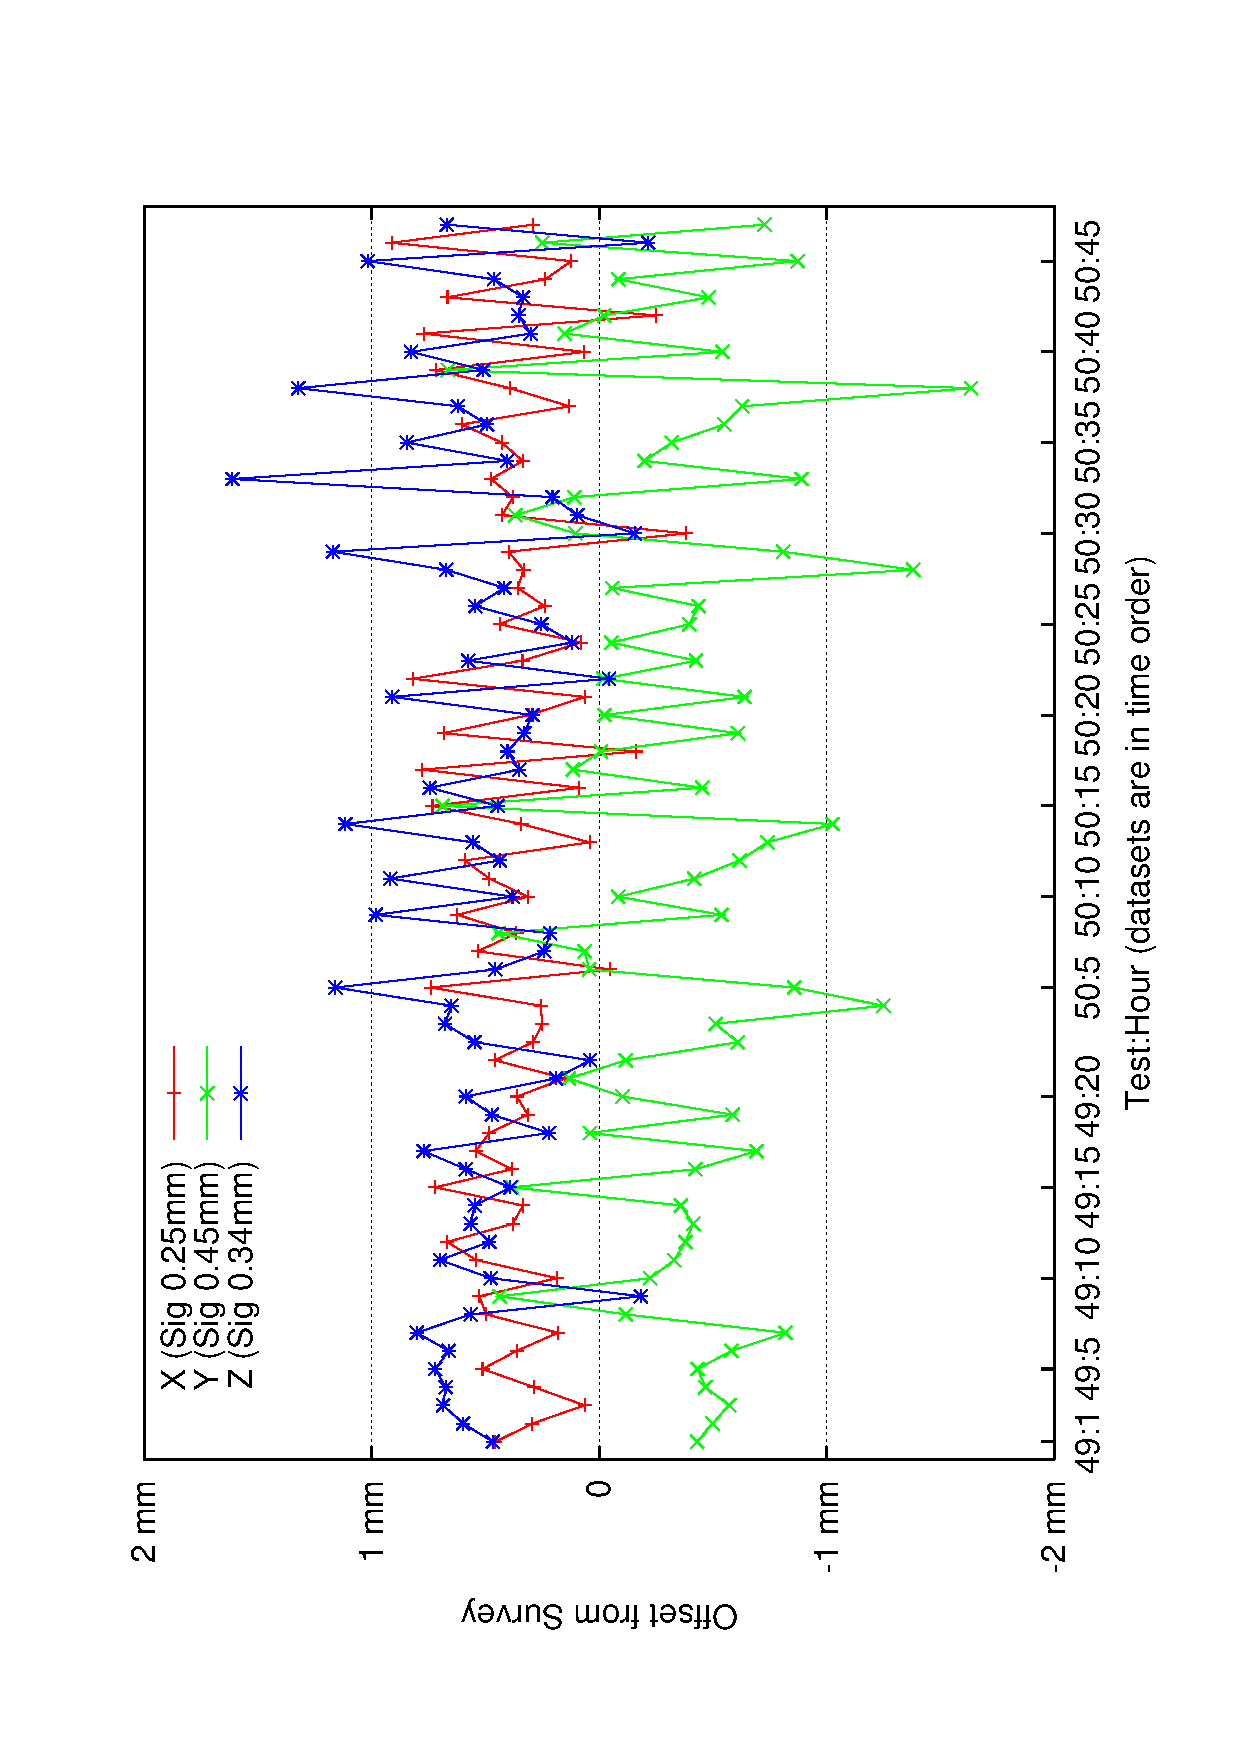
\includegraphics[width=7cm,angle=-90]{Fig1ION06}
   }

   \subfigure[From 21 hour survey, 5 kilometer baseline]{
      \label{fig:bt2}
      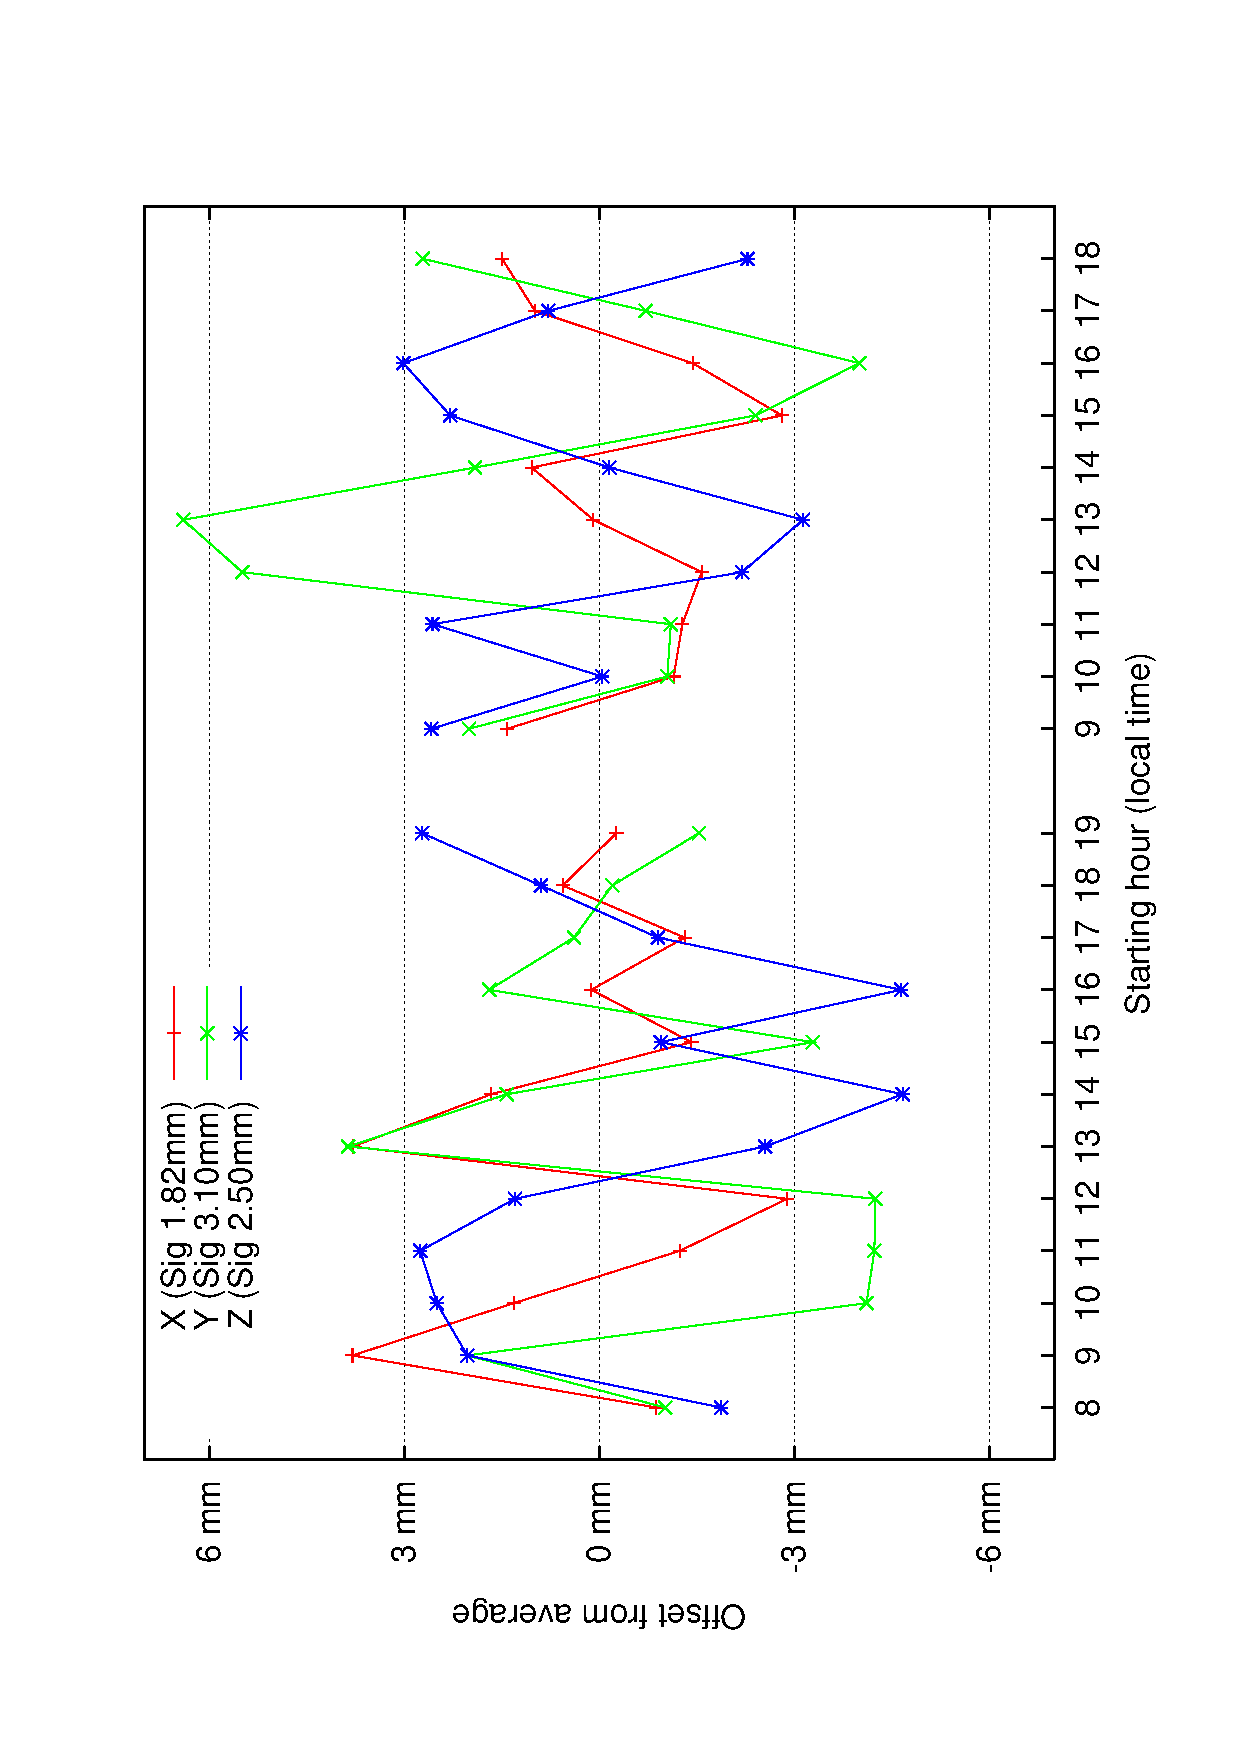
\includegraphics[width=7cm,angle=-90]{Fig2ION06}
   }

   \subfigure[From 21 hour survey, 5 kilometer baseline, 
              in overlapping 3-hour datasets] {
      \label{fig:bt3}
      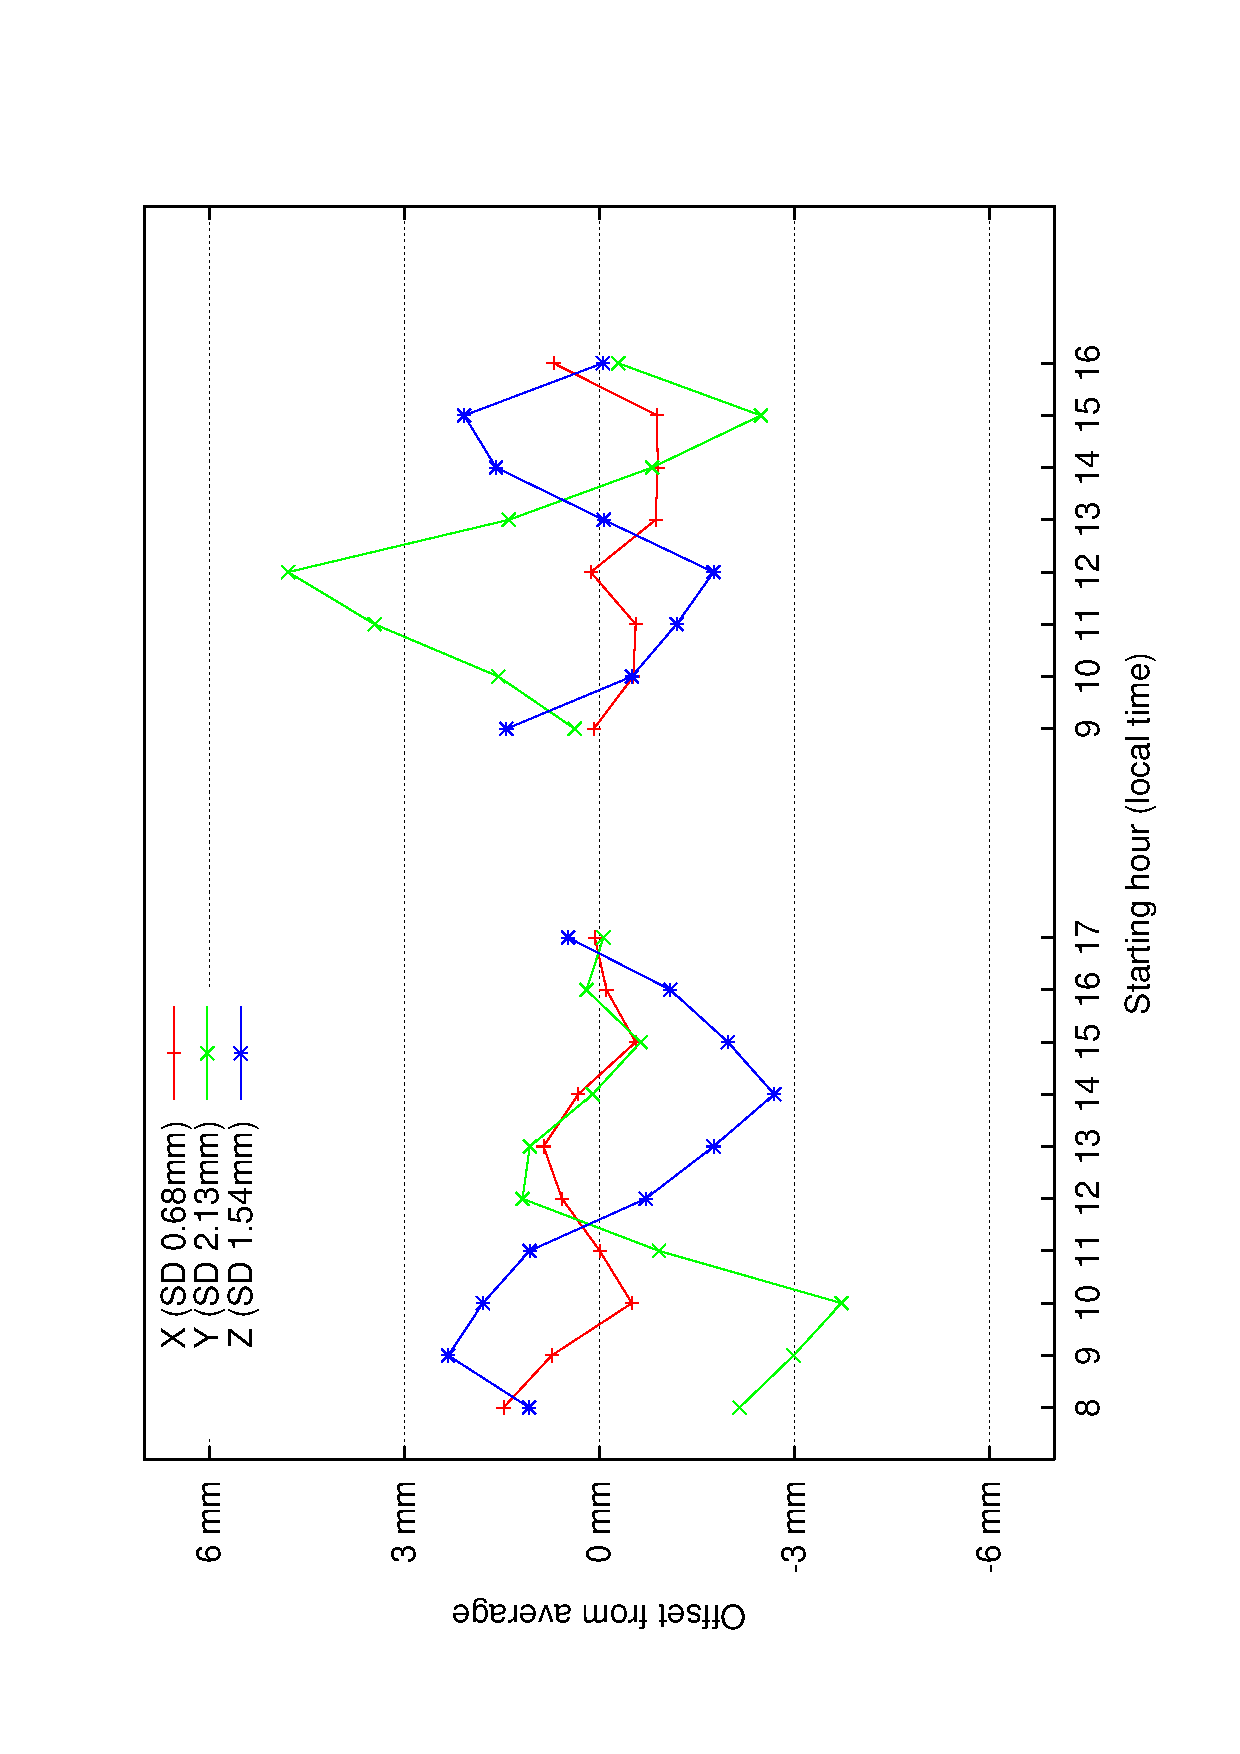
\includegraphics[width=7cm,angle=-90]{Fig3ION06}
   }

   \caption{\gpstkapplication{DDBase} position solution residuals}

\end{figure*}

Improvement and further development of \gpstkapplication{DDBase} is
continuing. ARL:UT is actively using \gpstkapplication{DDBase} to work
on the measurement of antenna phase center variations (PCV), including
ways to input more detailed (such as tabular) PCV data into
\gpstkapplication{DDBase}. ARL:UT also continues to test
\gpstkapplication{DDBase} at longer baselines and to implement new
features. We are also very interested in the identification and
mitigation of multipath within \gpstkapplication{DDBase}. We look
forward to interest and involvement in \gpstkapplication{DDBase} from
the GPSTk community.

\section*{Library Functions}

The GPSTk library has been enhanced since the last presentation at the
ION. The code base has been modified to support GNU GCC C++
(gcc) version 4. Also, the library has been modified to support native
64 bit Linux. Many contributions, including two major ones, have been added. The
library can now read and write low level BINEX streams.  New ways
to represent and store time have been prototyped. There are many
smaller contributions that would be of interest to the general
community.

\subsection*{Low Level BINEX Support}

BINEX is a binary format for the exchange of GPS/GLONASS/SBAS
data \cite{binexformat}. The design of BINEX is ongoing and emphasizes
flexibility and extensibility. Due to the increasing relevance of
BINEX, the GPSTk has been updated to support it. Like BINEX
itself, support for BINEX in the GPSTk is still evolving.

BINEX support in the GPSTk facilitates the reading and writing of
files containing generic BINEX records and accessing of data in
those records.  The support mirrors that provided for other
record-based formats in the toolkit.  Two new classes are provided,
one to represent an individual record and one to represent a stream of
records.

\begin{itemize}
   \item{ \gpstkclass{BinexData}. This derivative of \gpstkclass{FFData} 
          encapsulates an individual BINEX record and provides methods for 
          safely accessing record contents. This class includes subclasses 
          \gpstkclass{UBNXI} and \gpstkclass{MGFZI} to represent 
           BINEX values of the same name.}
   \item{ \gpstkclass{BinexStream}. This derivative of 
          \gpstkclass{FFBinaryStream} facilitates the reading and writing 
           of \gpstkclass{BinexData} objects to files. }
\end{itemize}

The implementation of BINEX support in the GPSTk adheres to the
object-oriented style of the toolkit while leveraging existing
prototype code from UNAVCO \cite{binexformat}.  In addition, the GPSTk implementation
features robust BINEX record validation, error handling, and
encapsulation.  Figure~\ref{fig:binexclasses} depicts the structure of
the new BINEX classes. The diagram follows the Unified Modeling
Language (UML) format \cite{umlstandard}.

\begin{figure*}[htbp]
  \centering
  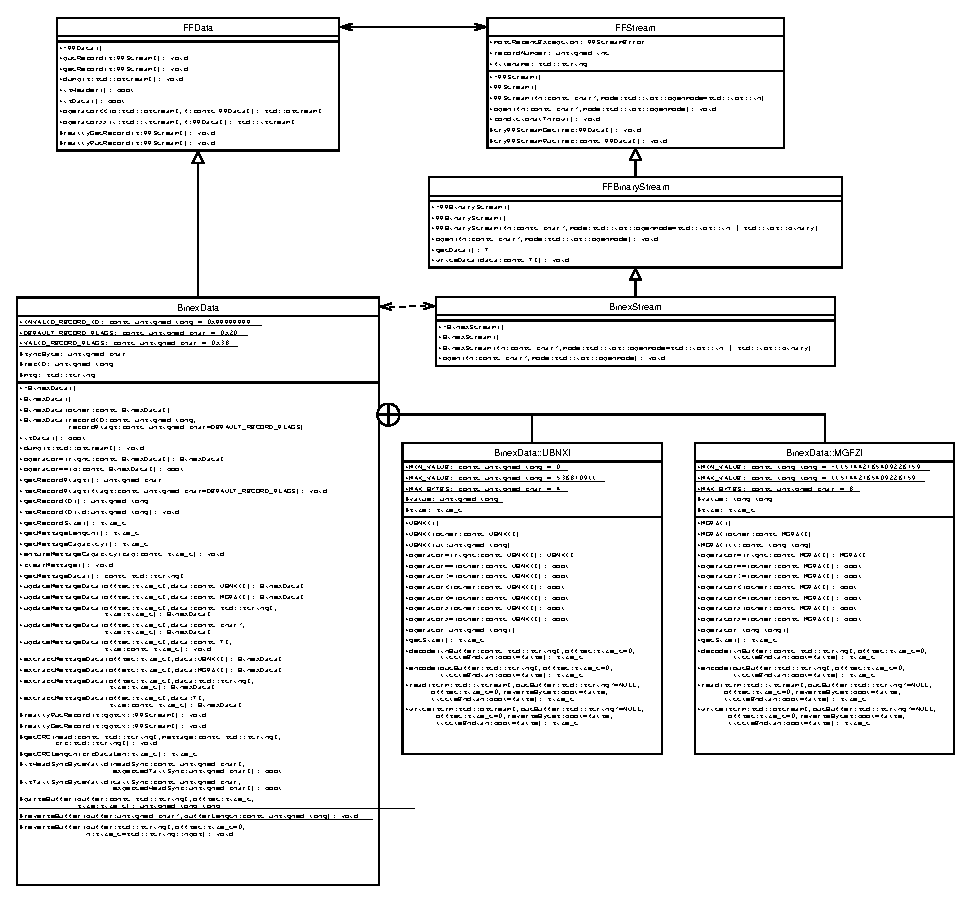
\includegraphics{binexgpstk}
  \caption{BINEX classes added to the GPSTk library}
  \label{fig:binexclasses}
\end{figure*}


Using the new BINEX classes is straightforward.  To read data from a
BINEX file, a user must first create and open a BinexStream then
repeatedly create BinexData objects filled with data from the stream.
Data can be extracted from the resulting objects at any later time.
This process is illustrated in Figure~\ref{fig:binexclientcode}.


\begin{figure*}[htbp]
%\renewcommand{\baselinestretch}{0.0}
\begin{small}
\begin{bf}
\begin{lstlisting}
#include "BinexData.hpp"
#include "BinexStream.hpp"

// Read a BINEX file and output the first 3 fields of message data for each record
// (assuming the fields are a long, a short, and a float).
//
int main (int argc, char *argv[])
{
   gpstk::BinexStream inStream("inputfile", std::ios::in | std::ios::binary);   
   inStream.exceptions(ios_base::failbit);
   while (inStream.good() && (EOF != inStream.peek() ) )
   {
      gpstk::BinexData record;
      try
      {
         record.getRecord(inStream);

         size_t offset = 0;
         long   field1;
         short  field2;
         float  field3;

         record.extractMessageData(offset, field1, sizeof(field1) );
         record.extractMessageData(offset, field2, sizeof(field2) );
         record.extractMessageData(offset, field3, sizeof(field3) );

         std::cout << "Data: " << field1 << ", " << field2 << ", "
                               << field3 << std::endl;
      }
      catch (gpstk::FFStreamError e)
      {
         std::cout << e << std::endl;
      }
      catch (...)
      {
         std::cout << "Unknown error reading record." << std::endl;
      }
   }
   inStream.close();
   return 0;
}

\end{lstlisting}
\end{bf}
\end{small}
\caption{Example of code using BINEX routines}
\label{fig:binexclientcode}
%\renewcommand{\baselinestretch}{1.0}
\end{figure*}

\subsection*{New Time Classes}
Most of the representations of time in the GPSTk library utilize the
\gpstkclass{DayTime} class. This single class is used to both convert
and store time quantities. Not only is \gpstkclass{DayTime} used to
note epochs, but also to correct pseudorange and phase observations for
known effects such as Earth rotation or clock drift. Therefore,
the precision of \gpstkclass{DayTime} directly limits the precision of corrected
observations. Furthermore, as \gpstkclass{DayTime} must convert most
time quantities at least once, there are round-off and truncation
errors associated with using time quantities in the GPSTk.

A new set of class has been prototyped that separate conversion from
storage. To promote a uniform interface to all time classes, the
new storage classes inherit from the class \gpstkclass{TimeTag}. For
example, the classes \gpstkclass{GPSWeekZcount} and \gpstkclass{MJD}
derive from \gpstkclass{TimeTag}. \gpstkclass{GPSWeekZcount}
uses two parameters to store an epoch: an \gpstkclass{int} for the GPS
week and an \gpstkclass{int} for Z-count. The class \gpstkclass{MJD}
uses only one parameter called a \gpstkclass{double}. Conversion among the new classes
is accomplished by converting to and from the intermediate class
\gpstkclass{CommonTime}.

At this time these classes are provided for evaluation. When this
approach has been assessed for usability and thoroughly tested, 
\gpstkclass{DayTime} will be replaced throughout the library in favor
of the new time classes. There will be a period of transition where
\gpstkclass{DayTime} is still provided for backwards compatibility.

\subsection*{Minor Changes}
Support for the RINEX version 2.11 standard has been added
\cite{rinex300format}. In addition to other changes, RINEX 2.11 introduces 
the L2C pseudorange observable \rinexobservable{C2}.  Other library 
enhancements apply to the processing of GNSS
observations in a general sense. New code has been added to convert
satellite positions from ECEF coordinates to a radial/alongtrack/crosstrack 
(RAC) coordinate system.


\section*{Future Directions}

The future capabilities of the GPSTk software suite depend wholly on
contributions. Within ARL:UT, improvements to the GPSTk are
underway. Some of these improvements are porting activities. Others
projects have identified specific new functionality.

Multiple projects within ARL:UT wish to make the \mbox{GPSTk} software
suite function on more operating systems using a larger variety of
compilers. Efforts are underway to create a full featured port to the
Mac OS X operating system. Also, the GPSTk is being ported to the
Borland C++ series of compilers, providing another choice to those who
wish to develop GPSTk based applications in Windows. Both Borland and Microsoft now offer free, lightweight versions of their commercial compilers \cite{borlandfreecompiler},
\cite{microsoftfreecompiler}. Support for both of those
compilers is a goal for the GPSTk project.

RINEX provides a widely
supported way to store GNSS data in a platform independent ASCII
format that has been in use since the late
1980s\cite{rinex1format}. RINEX~Version~3 includes a major change to the
format that is meant to handle the upcoming changes to GPS due to
modernization efforts and the upcoming Galileo system
\cite{rinex300format}. Version 3 maintains a similar ASCII format while
expanding the format to have more flexible and expandable
observation identifiers.  Internal ARL:UT projects have identified
that supporting this format will be useful.  ARL:UT intends to
integrate support of the format into a future version of the GPSTk.

\section*{Summary}

After two years of operation, the GPSTk has amassed a number of
contributions. Many contributions have enhanced the library to allow
for improved processing of observations or ephemerides. Many of these
contributions have taken the form of command line or console
applications. Those applications are now available not only as source
but also as binaries. These applications can be used in a
variety of stages in the research and development process.

\section*{Acknowledgments}
The authors would like to thank ARL:UT for its long term support of
the GPSTk project.  Also, they would like to thank the many members of
the GPSTk developer community that have assisted the project with
patches, applications, and bug reports to the GPSTk project. In
particular, Martin Vermeer and Dagoberto Salazar have made notable
contributions.

\begin{flushleft}

\bibliography{gpstk}
%\bibliographystyle{plain} % alphabetized
\bibliographystyle{unsrt}  % ordered by reference

\end{flushleft}

\end{document}
